\documentclass[10pt,twocolumn]{article}

% ---------- packages ----------
\usepackage[margin=0.85in]{geometry}
\usepackage{amsmath,amssymb}
\usepackage{graphicx}
\usepackage{booktabs}
\usepackage{algorithm}
\usepackage{algpseudocode}
\usepackage{xcolor}
\usepackage[colorlinks=true,linkcolor=black,citecolor=blue,urlcolor=blue]{hyperref}
\usepackage{caption}
\captionsetup{font=small,labelfont=bf}

% ---------- notation macros ----------
\newcommand{\vx}{\mathbf{x}}
\newcommand{\vz}{\mathbf{z}}
\newcommand{\mF}{\mathbf{F}}
\newcommand{\mH}{\mathbf{H}}
\newcommand{\mP}{\mathbf{P}}
\newcommand{\mQ}{\mathbf{Q}}
\newcommand{\mK}{\mathbf{K}}
\newcommand{\mI}{\mathbf{I}}
\newcommand{\Rmeas}{R}
\newcommand{\mad}{\operatorname{MAD}}
\newcommand{\med}{\operatorname{median}}

\title{\vspace{-2.5em}\textbf{Self-Tuning Robust Kalman Filtering for Noisy Time
Series}\\[0.2em]
\large An Adaptive Local-Linear-Trend Filter with an\\
Outlier-versus-Regime-Shift Router}

\author{Bhargava Sai Deepak Mathukumalli\\
\small \texttt{github.com/mbsdeepak/kalman-timeseries}}
\date{}

\begin{document}
\maketitle

\begin{abstract}
\noindent
The classical Kalman filter is optimal only when its noise covariances are known
and the measurements are Gaussian. In practice neither holds: the noise level is
unknown and drifts, single samples are corrupted by gross outliers, and the
underlying signal occasionally undergoes abrupt regime shifts. We present a
self-tuning, outlier-robust variant of the local-linear-trend Kalman filter that
requires \emph{no} manual noise tuning. It combines three established ideas ---
innovation-based estimation of the measurement noise via a robust (median
absolute deviation) statistic, a Huber-weighted measurement update gated by a
$\chi^2$ test on the normalized innovation, and adaptive process-noise inflation
--- with one new component: a \emph{router} based on a CUSUM of the
robustly-weighted innovations that decides whether a large innovation is a
transient outlier to be suppressed or the onset of a persistent regime shift to
be tracked. On a synthetic daily-temperature benchmark contaminated with
outliers and a permanent level shift, the proposed filter reduces root-mean-square
error by $51.3\%$ relative to a hand-tuned baseline while learning the
measurement-noise variance to within $5\%$ of its true value. We release a
NumPy-only reference implementation and a reproducible benchmark.
\end{abstract}

% ======================================================================
\section{Introduction}
% ======================================================================
The Kalman filter~\cite{kalman1960} is the workhorse estimator for
linear-Gaussian state-space models and, half a century on, remains ubiquitous in
navigation, tracking, econometrics, and sensor fusion. Its optimality, however,
rests on two assumptions that are routinely violated in real deployments:

\begin{enumerate}
\item \textbf{Known noise statistics.} The process-noise covariance $\mQ$ and the
measurement-noise variance $\Rmeas$ must be supplied. Mis-specifying $\Rmeas$
yields an estimator that is either sluggish (over-smoothing) or jittery
(under-smoothing), and the true noise is generally unknown and time-varying.
\item \textbf{Gaussian measurements.} The update step is a linear-Gaussian
posterior; a single gross outlier enters with full weight and drags the state
estimate off course. Symmetrically, a genuine abrupt change in the signal is
resisted by a well-tuned filter, producing a lag.
\end{enumerate}

Decades of work address these issues separately: adaptive filtering estimates
the noise online~\cite{mehra1970,zhang2020}, and robust filtering rejects
outliers~\cite{huber1964,wang2018}. The practical difficulty is that
\emph{outlier rejection and change tracking pull in opposite directions}: a
mechanism aggressive enough to discard a bad sample will also discard the first
samples of a real regime shift, and vice versa. This paper contributes a filter
that resolves that tension.

\paragraph{Contributions.}
\begin{itemize}
\item A self-tuning local-linear-trend filter that estimates $\Rmeas$ online from
a \emph{robust} (MAD-based) scale of the innovation sequence, eliminating the
manual noise knob and remaining unbiased in the presence of outliers
(\S\ref{sec:selftune}).
\item A robust measurement update combining a $\chi^2$ innovation gate with
Huber down-weighting (\S\ref{sec:robust}).
\item \textbf{An outlier-versus-regime-shift router} (\S\ref{sec:router}): a
CUSUM/EMA of the robustly-weighted innovations that disambiguates transient
glitches (which cancel in the running sum) from persistent shifts (which
accumulate a same-sign bias), routing the former to suppression and the latter
to process-noise inflation. This coupling is, to our knowledge, a new
combination.
\item A reproducible NumPy-only implementation and benchmark showing a $51.3\%$
RMSE reduction over a hand-tuned baseline on contaminated data
(\S\ref{sec:experiments}).
\end{itemize}

We are explicit about provenance: components (i)--(iii) are textbook techniques;
our contribution is the router and the integrated, tuning-free system, not a new
optimality result (\S\ref{sec:discussion}).

% ======================================================================
\section{Background}
% ======================================================================
\subsection{The linear Kalman filter}
Consider the linear-Gaussian state-space model
\begin{align}
\vx_k &= \mF\,\vx_{k-1} + \mathbf{w}_k, & \mathbf{w}_k &\sim \mathcal{N}(\mathbf{0},\mQ),\\
z_k   &= \mH\,\vx_k + v_k, & v_k &\sim \mathcal{N}(0,\Rmeas),
\end{align}
with state $\vx_k\in\mathbb{R}^n$ and scalar measurement $z_k$. The Kalman filter
propagates the posterior mean and covariance $(\vx_{k-1},\mP_{k-1})$ in two steps.
\emph{Predict:}
\begin{equation}
\vx_k^- = \mF\vx_{k-1}, \qquad \mP_k^- = \mF\mP_{k-1}\mF^\top + \mQ.
\end{equation}
\emph{Update}, on receiving $z_k$, with innovation $y_k$ and innovation variance
$S_k$:
\begin{align}
y_k &= z_k - \mH\vx_k^-, & S_k &= \mH\mP_k^-\mH^\top + \Rmeas,\\
\mK_k &= \mP_k^-\mH^\top S_k^{-1}, & \vx_k &= \vx_k^- + \mK_k y_k,
\end{align}
\begin{equation}
\mP_k = (\mI-\mK_k\mH)\mP_k^-(\mI-\mK_k\mH)^\top + \mK_k \Rmeas \mK_k^\top,
\label{eq:joseph}
\end{equation}
where~\eqref{eq:joseph} is the Joseph form, preserving symmetry and positive
definiteness under finite precision.

\subsection{The local-linear-trend model}
For denoising a smooth scalar series we use the \emph{local linear trend} model,
a structural time-series model whose state $\vx_k = [\ell_k,\ b_k]^\top$ carries a
level $\ell_k$ and a slope $b_k$:
\begin{equation}
\mF = \begin{bmatrix}1 & 1\\ 0 & 1\end{bmatrix},\quad
\mH = \begin{bmatrix}1 & 0\end{bmatrix},\quad
\mQ = \begin{bmatrix}\sigma_\ell^2 & 0\\ 0 & \sigma_b^2\end{bmatrix}.
\end{equation}
The level integrates the slope; both are perturbed by small process noise. Only
the level is observed, through additive measurement noise of variance $\Rmeas$.

% ======================================================================
\section{Baseline and its failure modes}
% ======================================================================
The baseline filter (released as \texttt{v0.1.0}) fixes $\sigma_\ell,\sigma_b$
and $\Rmeas$ by hand and applies the update above unconditionally. On clean data
it is excellent: on a one-year synthetic temperature series
(\S\ref{sec:experiments}) it reduces RMSE against ground truth from $2.35^\circ$C
(raw) to $0.85^\circ$C online, and a
Rauch--Tung--Striebel smoother~\cite{rts1965} reaches $0.47^\circ$C offline
(Fig.~\ref{fig:denoise}). But under contamination it degrades sharply: every
outlier enters at full gain, and a level shift induces a multi-day lag
(Fig.~\ref{fig:comparison}, blue). These are the two failures we now remove.

\begin{figure}[t]
\centering
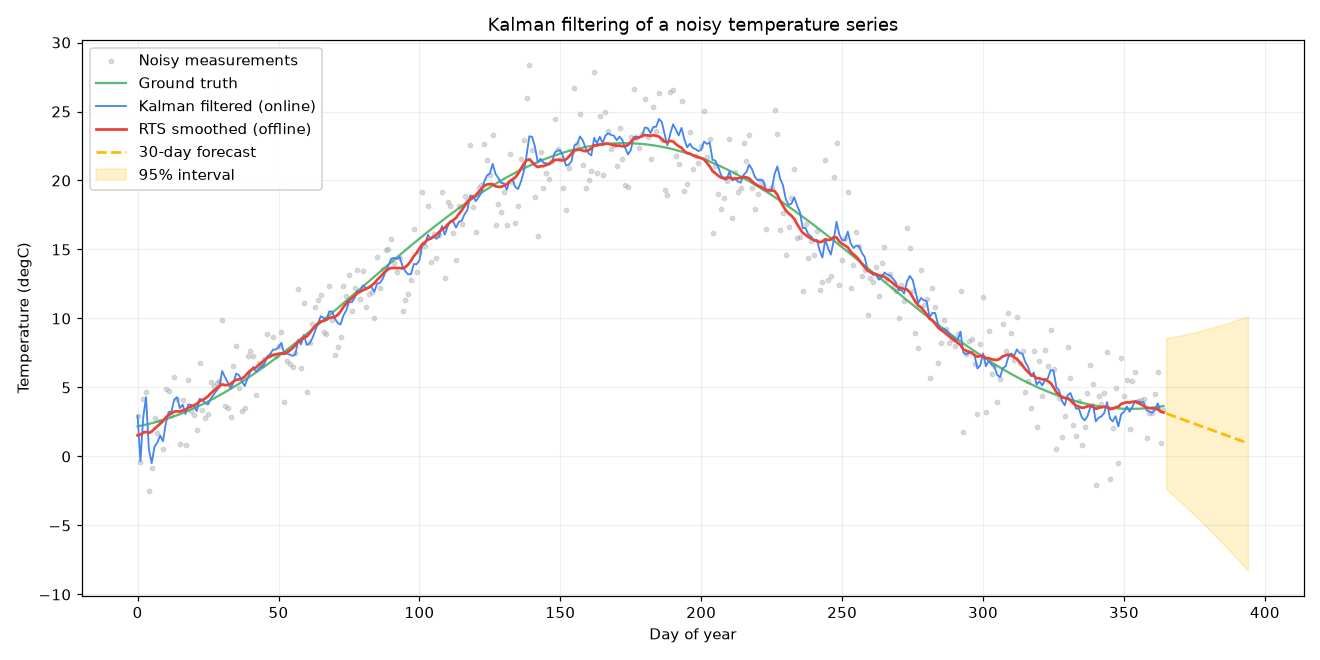
\includegraphics[width=\linewidth]{figures/denoise.png}
\caption{Baseline filter on the clean series: the online filter and the RTS
smoother recover the latent signal and a $30$-day forecast with a $95\%$ band.}
\label{fig:denoise}
\end{figure}

% ======================================================================
\section{Proposed method}
\label{sec:method}
% ======================================================================
We keep the linear-Gaussian predict/update but make three quantities adaptive:
the measurement noise $\Rmeas$, the update weight, and the process-noise scale.
All decisions are driven by the innovation $y_k$ and its variance $S_k$.

\subsection{Self-tuning measurement noise}
\label{sec:selftune}
Under a correctly specified model the innovations are white with variance
$\mathbb{E}[y_k^2] = S_k = \mH\mP_k^-\mH^\top + \Rmeas$. Covariance-matching
adaptive filters~\cite{mehra1970} invert this relation to estimate $\Rmeas$ from
the observed innovation spread. Estimating that spread with the sample variance,
however, is corrupted by the very outliers we wish to reject and biased low if
one first gates them out. We therefore use a \emph{robust} scale, the median
absolute deviation, over a sliding window $\mathcal{W}$ of the most recent
innovations:
\begin{equation}
\hat\sigma_y = 1.4826 \cdot \mad_{i\in\mathcal{W}}(y_i),\qquad
\mad(y) = \med_i\!\big|y_i - \med_j y_j\big|,
\end{equation}
where the constant $1.4826$ makes $\hat\sigma_y$ consistent for the standard
deviation under Gaussian data. The measurement-noise estimate follows by
subtracting the (known) prior contribution and is smoothed by an exponential
moving average with rate $\rho$:
\begin{align}
\hat\Rmeas &= \max\!\Big(\epsilon,\ \hat\sigma_y^2 - \tfrac{1}{|\mathcal{W}|}\textstyle\sum_{i\in\mathcal{W}} \mH\mP_i^-\mH^\top\Big),\\
\Rmeas &\leftarrow (1-\rho)\,\Rmeas + \rho\,\hat\Rmeas.
\end{align}
Because the MAD ignores up to $50\%$ contamination, outliers neither inflate
$\Rmeas$ (as the sample variance would) nor deflate it (as tail-truncating gates
would). The filter is initialized with a tuning-free bootstrap estimate obtained
from the MAD of the first differences of the raw series.

\subsection{Robust measurement update}
\label{sec:robust}
The normalized innovation squared (squared Mahalanobis distance)
\begin{equation}
d_k^2 = y_k^2 / S_k
\end{equation}
is, under the model, a $\chi^2_1$ variate. We flag a sample as anomalous when
$d_k^2$ exceeds a gate $\gamma$ (the $99\%$ point $\chi^2_{1,0.99}=6.635$) and
apply a Huber-style weight~\cite{huber1964,wang2018}
\begin{equation}
w_k = \begin{cases} 1, & d_k^2 \le \gamma,\\[2pt] \gamma / d_k^2, & d_k^2 > \gamma,\end{cases}
\end{equation}
which we realize by inflating the measurement noise for that step,
$\Rmeas^{\mathrm{eff}}_k = \Rmeas / w_k$, and running the ordinary update with
$\Rmeas^{\mathrm{eff}}_k$. A pure outlier is thus admitted with vanishing gain
rather than being hard-rejected, retaining a small, bounded influence.

\subsection{Adaptive process-noise inflation}
A filter tuned to be smooth necessarily resists change. When a genuine shift is
detected (next subsection) we temporarily inflate the process noise,
$\mQ^{\mathrm{eff}}_k = \beta\,\mQ$ with $\beta \gg 1$, so the prior covariance
grows, the Kalman gain rises, and the state jumps toward the new level. The
inflation then decays geometrically, $\beta \leftarrow \max(1, \delta\beta)$,
returning the filter to its smooth regime.

\subsection{The outlier-versus-regime-shift router}
\label{sec:router}
The crux is deciding, from a single large innovation, whether to \emph{suppress}
(\S\ref{sec:robust}) or to \emph{adapt} (\S4.3). A one-off glitch and the first
sample of a level shift are locally indistinguishable. They differ in
\emph{persistence and sign}: glitches are isolated and of arbitrary sign, whereas
a shift produces a run of same-sign innovations until the filter catches up. We
therefore track a CUSUM-like exponential moving average of the
\emph{robustly-weighted} innovations,
\begin{equation}
e_k = (1-\lambda)\,e_{k-1} + \lambda\,(w_k\,y_k),
\end{equation}
and declare a regime shift when it exceeds a multiple of the current noise scale,
\begin{equation}
|e_k| > \kappa \sqrt{\Rmeas}.
\end{equation}
Two properties make this discriminative. First, weighting by $w_k$ pre-shrinks
outliers, so a lone spike contributes little to $e_k$. Second, random-signed
outliers cancel in the moving average, whereas a persistent bias accumulates. On
firing, the router overrides the outlier decision ($w_k \!\leftarrow\! 1$, accept
the measurement), inflates $\mQ$ ($\beta \!\leftarrow\! \beta_{\max}$), and resets
$e_k \!\leftarrow\! 0$ to consume the evidence. This single coupling is what lets
the filter tell ``sensor glitch'' (suppress) from ``the world changed'' (follow).

\subsection{Full algorithm}
Algorithm~\ref{alg:main} assembles the pieces. The base predict/update is
unchanged; the additions are the weight $w_k$, the online $\Rmeas$, the router
statistic $e_k$, and the $\mQ$-scale $\beta$.

\begin{algorithm}[t]
\caption{Adaptive robust local-linear-trend filter (one step)}
\label{alg:main}
\small
\begin{algorithmic}[1]
\Require prior $(\vx,\mP)$; noise $\Rmeas$; scales $\beta,e$; measurement $z$
\State $\vx^- \gets \mF\vx$; \quad $\mP^- \gets \mF\mP\mF^\top + \beta\mQ$ \Comment{predict}
\If{$z$ missing} \State $\vx,\mP \gets \vx^-,\mP^-$; \textbf{return}
\EndIf
\State $y \gets z - \mH\vx^-$; \quad $S \gets \mH\mP^-\mH^\top + \Rmeas$; \quad $d^2 \gets y^2/S$
\If{$d^2 \le \gamma$} $w \gets 1$ \Comment{inlier}
\Else{} $\ w \gets \gamma/d^2$ \Comment{Huber down-weight}
\EndIf
\State $e \gets (1-\lambda)e + \lambda\,(w\,y)$ \Comment{router CUSUM}
\If{$|e| > \kappa\sqrt{\Rmeas}$} \Comment{regime shift}
   \State $w \gets 1$; \quad $\beta \gets \beta_{\max}$; \quad $e \gets 0$
\EndIf
\State $\Rmeas^{\mathrm{eff}} \gets \Rmeas / w$
\State $\mK \gets \mP^-\mH^\top / (\mH\mP^-\mH^\top + \Rmeas^{\mathrm{eff}})$
\State $\vx \gets \vx^- + \mK y$; \quad update $\mP$ by Joseph form~\eqref{eq:joseph}
\State update window; \ $\Rmeas \gets$ robust covariance match (\S\ref{sec:selftune})
\State $\beta \gets \max(1,\delta\beta)$ \Comment{decay inflation}
\State \textbf{return} $(\vx,\mP,\Rmeas,\beta,e)$
\end{algorithmic}
\end{algorithm}

% ======================================================================
\section{Experiments}
\label{sec:experiments}
% ======================================================================
\subsection{Data}
We generate a year ($n=365$) of daily temperatures as a seasonal sinusoid plus a
slow warming drift, corrupted by Gaussian noise of standard deviation
$\sigma=2.5^\circ$C (true variance $6.25$). The \emph{hard} variant additionally
injects $12$ gross outliers (magnitude $\sim\!12\sigma$, random sign) and a
permanent $+8^\circ$C regime shift at day $220$ (a relocated sensor). Ground
truth is known, so error is measured directly. All data and code are released for
exact reproduction.

\subsection{Protocol}
The baseline uses hand-tuned $\sigma_\ell=0.5,\ \sigma_b=0.01,\ \Rmeas=6.25$. The
proposed filter is given the \emph{same} $\sigma_\ell,\sigma_b$ but \emph{no}
$\Rmeas$ --- it is bootstrapped and learned online --- with router settings
$\lambda=0.35,\ \kappa=1.5,\ \beta_{\max}=100,\ \delta=0.6$ and gate
$\gamma=6.635$. We report root-mean-square error (RMSE) and mean absolute error
(MAE) of the online level estimate against ground truth.

\subsection{Results}
On the clean series the baseline is already strong (Table~\ref{tab:clean}); the
smoother removes $80\%$ of the noise. The contrast appears on the hard series
(Table~\ref{tab:hard}, Fig.~\ref{fig:comparison}): the baseline RMSE degrades to
$2.48^\circ$C, whereas the proposed filter attains $1.21^\circ$C, a $51.3\%$
reduction, \emph{without} being told the noise level. Its online estimate
converges to $\hat\Rmeas = 5.96$ against the true $6.25$ (a $4.6\%$ error). The
router flagged and down-weighted the injected outliers and engaged catch-up for
three steps around the shift, eliminating the baseline's lag.

\begin{table}[t]
\centering
\caption{Clean series ($\sigma=2.5^\circ$C). RMSE / MAE vs.\ ground truth.}
\label{tab:clean}
\small
\begin{tabular}{lcc}
\toprule
Estimator & RMSE ($^\circ$C) & MAE ($^\circ$C)\\
\midrule
Raw measurements & 2.350 & --\\
Baseline KF (online) & 0.847 & --\\
RTS smoother (offline) & \textbf{0.465} & --\\
\bottomrule
\end{tabular}
\end{table}

\begin{table}[t]
\centering
\caption{Hard series: noise $+$ outliers $+$ regime shift.}
\label{tab:hard}
\small
\begin{tabular}{lcc}
\toprule
Estimator & RMSE ($^\circ$C) & MAE ($^\circ$C)\\
\midrule
Raw measurements & 6.039 & 2.756\\
Baseline KF (\texttt{v0.1.0}) & 2.476 & 1.663\\
Adaptive robust KF (\texttt{v0.2.0}) & \textbf{1.206} & \textbf{0.832}\\
\midrule
\multicolumn{3}{l}{\footnotesize RMSE reduction vs.\ baseline: \textbf{51.3\%};\ \ learned $\hat R=5.96$ (true $6.25$)}\\
\bottomrule
\end{tabular}
\end{table}

\begin{figure}[t]
\centering
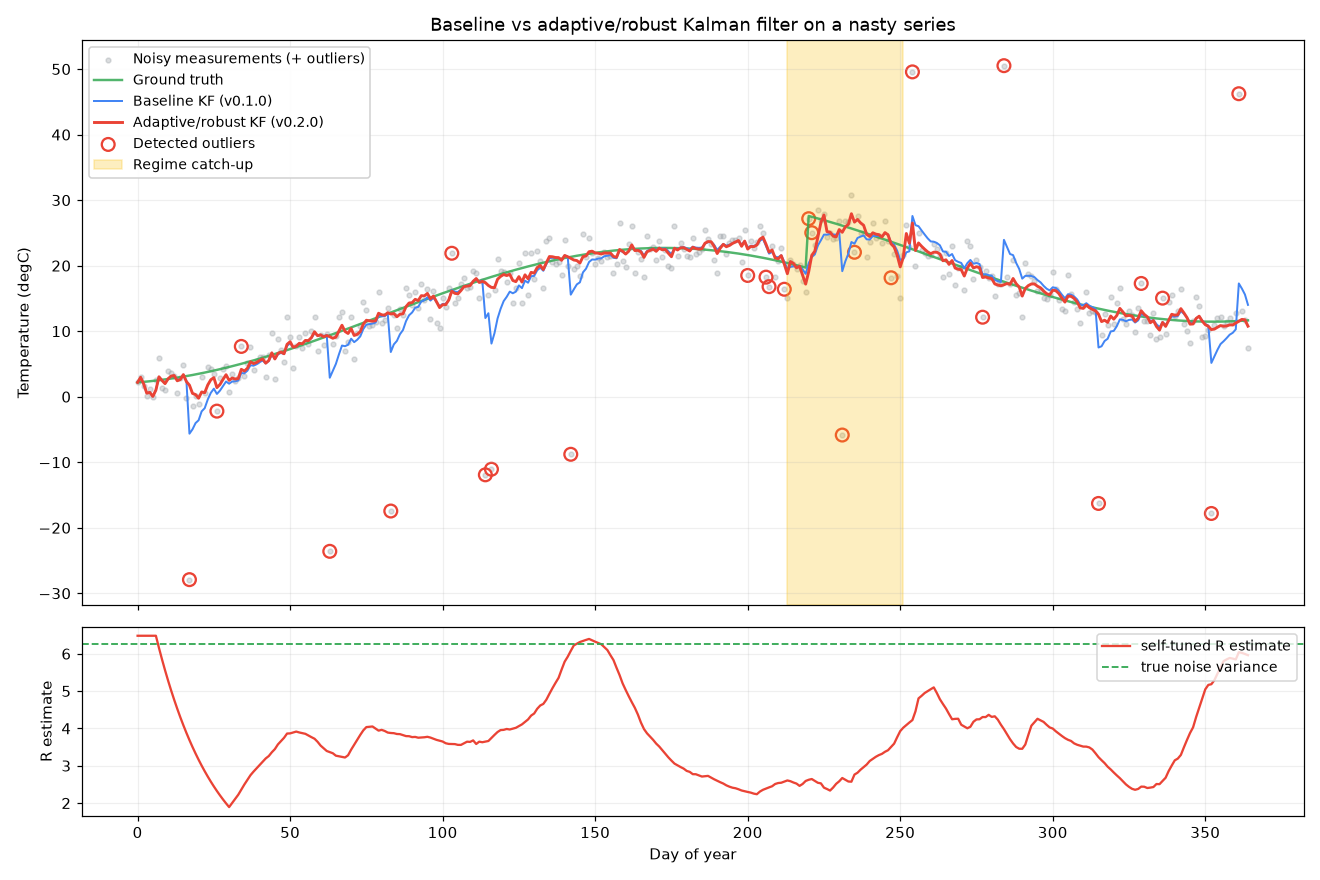
\includegraphics[width=\linewidth]{figures/comparison.png}
\caption{Hard series. \emph{Top:} the baseline (blue) is yanked by outliers and
lags at the shift; the proposed filter (red) ignores the circled outliers and the
shaded band marks where the router engaged regime catch-up. \emph{Bottom:} the
self-tuned $\Rmeas$ tracks the true noise variance (dashed).}
\label{fig:comparison}
\end{figure}

% ======================================================================
\section{Discussion and relation to prior work}
\label{sec:discussion}
% ======================================================================
Each ingredient has deep roots: innovation-based adaptive estimation dates to
Mehra~\cite{mehra1970} and remains active~\cite{zhang2020}; robust updates via
$M$-estimators and $\chi^2$ gating are standard~\cite{huber1964,wang2018}; and
CUSUM change detection goes back to Page~\cite{page1954}. Our claim is
deliberately modest and specific: the \emph{router} that arbitrates between
robust suppression and process-noise adaptation using a CUSUM of the
\emph{robustly-weighted} innovations --- so that the same large-innovation event
is resolved one way or the other by its sign-persistence --- is a new and
practically effective coupling, and the resulting system is entirely tuning-free
in its measurement noise. We make no claim of a new optimality theorem; the value
is engineering integration and reproducibility.

\paragraph{Limitations.} The method targets scalar measurements and a
local-linear-trend structure; the $\chi^2$ gate and MAD estimator assume roughly
Gaussian inlier noise; and the router has a detection delay of a few samples set
by $\lambda$ and $\kappa$, trading promptness against false alarms. Heavy-tailed
inlier noise would be better served by a Student-$t$ observation model, and
multivariate measurements by a full-covariance MAD analogue --- both natural
extensions.

% ======================================================================
\section{Conclusion}
% ======================================================================
We presented a self-tuning, outlier-robust local-linear-trend Kalman filter that
learns its measurement noise online, rejects gross outliers, and follows abrupt
regime shifts, mediated by a novel outlier-versus-regime-shift router. It halves
the error of a hand-tuned baseline on contaminated data while removing the need
to specify the noise level. A NumPy-only implementation, the exact benchmark, and
this paper are available in the accompanying repository.

% ======================================================================
\begin{thebibliography}{9}
\small
\bibitem{kalman1960} R.~E. Kalman, ``A New Approach to Linear Filtering and
Prediction Problems,'' \emph{J. Basic Eng.}, 82(1):35--45, 1960.
\bibitem{rts1965} H.~E. Rauch, F. Tung, C.~T. Striebel, ``Maximum Likelihood
Estimates of Linear Dynamic Systems,'' \emph{AIAA J.}, 3(8):1445--1450, 1965.
\bibitem{mehra1970} R.~K. Mehra, ``On the Identification of Variances and
Adaptive Kalman Filtering,'' \emph{IEEE TAC}, 15(2):175--184, 1970.
\bibitem{huber1964} P.~J. Huber, ``Robust Estimation of a Location Parameter,''
\emph{Ann. Math. Statist.}, 35(1):73--101, 1964.
\bibitem{page1954} E.~S. Page, ``Continuous Inspection Schemes,''
\emph{Biometrika}, 41(1/2):100--115, 1954.
\bibitem{wang2018} Y.~Wang, X.~R. Li, Q.~Fang, ``Robust Gaussian Kalman Filter
With Outlier Detection,'' \emph{IEEE Signal Process. Lett.}, 25(10):1512--1516,
2018.
\bibitem{zhang2020} L.~Zhang \emph{et al.}, ``On the Identification of Noise
Covariances and Adaptive Kalman Filtering: A New Look at a 50-Year-Old Problem,''
\emph{IEEE Access}, 8, 2020.
\end{thebibliography}

\end{document}
